%%
% The BIThesis Template for Bachelor Graduation Thesis
%
% 北京理工大学毕业设计(论文)第一章节 —— 使用 XeLaTeX 编译
%
% Copyright 2020-2023 BITNP
%
% This work may be distributed and/or modified under the
% conditions of the LaTeX Project Public License, either version 1.3
% of this license or (at your option) any later version.
% The latest version of this license is in
%   http://www.latex-project.org/lppl.txt
% and version 1.3 or later is part of all distributions of LaTeX
% version 2005/12/01 or later.
%
% This work has the LPPL maintenance status `maintained'.
%
% The Current Maintainer of this work is Feng Kaiyu.
%
% 第八章节

\chapter{实验结果}
% {本章将设计实验测试系统的性能、安全性和健壮性,并对比不同情况下对系统性能的影响,探讨系统的适用范围与最佳配置。}
\section{实验设计}
\subsection{实验数据采集}
{我们使用一台huawei mate40 pro进行数据采集,摄像头为1300万像素,分别采集帧率分别为30fps、60fps和分辨率分别为720p、1080p、4k的数据共6组进行对比,另外采集不同手指按压的数据研究不同手指按压对系统的影响。}

\par
\subsection{评估指标}
{本系统旨在为智能移动设备提供一种可靠安全的用户验证功能,为了评估系统的性能,我们定义一下参数:}
\begin{itemize}
    \item {真阳性率(true positive rate,TPR):} {又称敏感度(sensitivity,SEN),即实际有病而按该筛检试验的标准被正确地判为有病的百分比。它反映筛检试验发现病人的能力。在本实验中表现为合法用户验证成功的概率。}
    \item {假阳性率(false positive rate,FPR):} {又称误诊率,即实际无病,但根据筛检被判为有病的百分比。在本实验中表现为非法用户验证成功的概率。}
    \item {真阴性率(true negative rate,TNR):} {特定疾病诊断中,某方法认为特定人群中未患病人数(阴性数)与经病理检查或其他公认可信证据证实该人群中真实的未患病人数(阴性数)之比。反映该方法排除该疾病的能力。在本实验中表现为非法用户验证失败的概率。}
    \item {假阴性率(false negative rate,FNR):} {又称漏诊率,是指实际有病,但根据筛检试验被定为无病的百分比。在本实验中表现为合法用户验证失败的概率。}
\end{itemize}
{其中TNR=1-FPR,TPR=1-FNR,TNR与TPR越高,验证效果越好,否则则效果越差;FPR与FNR越低,验证效果越好,否则则效果越差。}
\par
\subsection{测试方法}
{我们在系统参数分别为$\gamma=5$,$\eta=0.9$的条件下进行测试,采集不同帧率、分辨率配置的摄像头录制的数据,同时在帧率为30fps,分辨率为1080p的条件下采集食指和中指按压摄像头的视频流进行对比测试。}
\par
{对每一组数据进行测试时,同时测评该组数据在不同心动周期数内验证的准确率,使用YoudenJ作为测评指标,并寻找最佳验证所需心动周期数。}
\section{识别准确率分析}
\subsection{不同帧率与分辨率下的准确率分析}
\begin{itemize}


    \item {\bf{30fps720p}}{%30fps720p
{我们首先使用帧率为30fps和分辨率为720p的数据进行实验,在该条件下采集了70个合法用户的心波,心率为84,70个心波提取的特征经过PCA转换后得到33个特征,用于测试的受试者采集的数据信息如表4-1所示,其中志愿者1为合法用户,其他为攻击用户。}
  \begin{table}[!ht]
    \linespread{1.5}
    \zihao{5}
	  \centering  % 显示位置为中间
	  \caption{受试者基本信息}  % 表格标题
	  \label{table4-1} 
	  %字母的个数对应列数,|代表分割线
	  % l代表左对齐,c代表居中,r代表右对齐
	  \scalebox{0.8}{\begin{tabular}{*{3}{>{\centering\arraybackslash}p{3cm}}} \toprule %l左对齐;c居中;r右对齐
	  	用户 & 心跳周期数 & 心率(单位: 次/min)   \\
	  	\hline
	  	志愿者1 & 33 & 83   \\
	  	志愿者2 & 28 & 81   \\
	  	志愿者3 & 21 & 85   \\
	  	志愿者4 & 32 & 111   \\
	  	志愿者5 & 15 & 97  \\
    \bottomrule
	  \end{tabular}}
  \end{table}

\par
{各个评估指标在不同心动周期作为验证步长的情况下测量值如表4-2所示。}

\begin{table*}[htbp]
  \linespread{1.5}
  \vspace{1cm}
  \zihao{5}
  \centering
  \caption{各参数实验结果统计表} 
\label{table4-2}
\scalebox{0.6}{
  \begin{tabular}{*{10}{>{\centering\arraybackslash}p{2cm}}} \toprule
  步长$n$ & 实际TPR & 理论TPR & 实际FNR & 理论FNR  & 实际TNR & 理论TNR & 实际FPR & 理论FPR & YoudenJ \\
    \hline
1&0.8182&0.8182&0.1818&0.1818&0.8021&0.8021&0.1979&0.1979&0.6203 \\ 
2&0.6875&0.6694&0.3125&0.3306&0.9583&0.9608&0.0417&0.0392 &0.6458 \\ 
3&0.6364&0.5477&0.3636&0.4523&0.9688&0.9922&0.0312&0.0078&0.6052 \\ 
4&0.375&0.4481&0.625&0.5519&1.0&0.9985&0.0&0.0015&0.375 \\ 
5&0.3333&0.3666&0.6667&0.6334&1.0&0.9997&0.0&0.0003&0.3333 \\ 
6&0.2&0.3&0.8&0.7&1.0&0.9999&0.0&0.0001 &0.2 \\ 
7&0.5&0.2454&0.5&0.7546&1.0&1.0&0.0&0.0&0.5 \\ 
8&0.25&0.2008&0.75&0.7992&1.0&1.0&0.0&0.0&0.25 \\ 
9&0.3333&0.1643&0.6667&0.8357&1.0&1.0&0.0&0.0&0.3333 \\ 
10&0.0&0.1344&1.0&0.8656&1.0&1.0&0.0&0.0&0.0 \\ 
\bottomrule
    \end{tabular}}
\end{table*}


\begin{figure}[H]
  \centering
  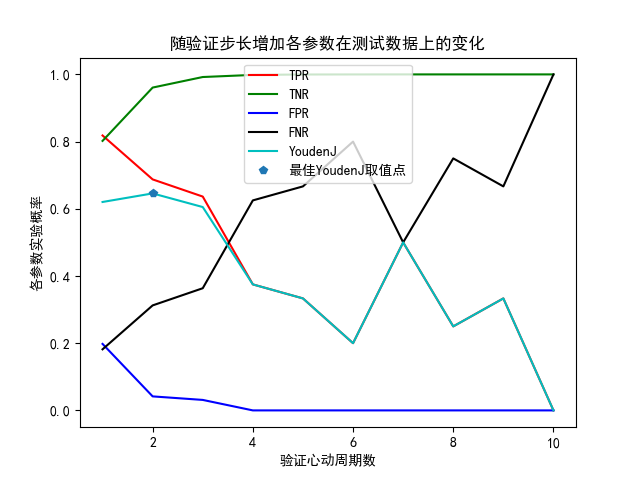
\includegraphics[width=0.7\linewidth]{images/30fps720p.png}
  \caption{30fps720p条件下各参数随验证所需心动周期数变化}\label{4-1} % label 用来在文中索引
\end{figure}

\par
{如图4-1所示,在心动周期数为2时取得最佳效果,此时的TPR为68.75\%,TNR为95.83\%。}}



\item {\bf{30fps1080p}}{%30fps1080p
{使用帧率为30fps和分辨率为1080p的数据进行实验,在该条件下采集了70个合法用户的心波,心率为67,70个心波提取的特征经过PCA转换后得到38个特征,用于测试的受试者采集的数据信息如表4-3所示,其中志愿者1为合法用户,其他为攻击用户。}
  \begin{table}[!ht]
    \linespread{1.5}
    \zihao{5}
	  \centering  % 显示位置为中间
	  \caption{受试者基本信息}  % 表格标题
	  \label{table4-3} 
	  %字母的个数对应列数,|代表分割线
	  % l代表左对齐,c代表居中,r代表右对齐
	  \scalebox{0.8}{\begin{tabular}{*{3}{>{\centering\arraybackslash}p{3cm}}} \toprule %l左对齐;c居中;r右对齐
	  	用户 & 心跳周期数 & 心率(单位: 次/min)   \\
	  	\hline
	  	志愿者1 & 50 & 73   \\
	  	志愿者2 & 30 & 87   \\
	  	志愿者3 & 21 & 82   \\
	  	志愿者4 & 29 & 91   \\
	  	志愿者5 & 27 & 77   \\
    \bottomrule
	  \end{tabular}}
  \end{table}
\par
{各个评估指标在不同心动周期作为验证步长的情况下测量值如表4-4所示。}
\begin{table*}[htbp]
  \linespread{1.5}
  \zihao{5}
  \centering
  \caption{各参数实验结果统计表} 
\label{table4-4}
\scalebox{0.6}{
  \begin{tabular}{*{10}{>{\centering\arraybackslash}p{2cm}}} \toprule
  步长$n$ & 实际TPR & 理论TPR & 实际FNR & 理论FNR  & 实际TNR & 理论TNR & 实际FPR & 理论FPR & YoudenJ \\
    \hline
1&0.94&0.94&0.06&0.06&0.7664&0.7664&0.2336&0.2336&0.7064 \\ 
2&0.88&0.8836&0.12&0.1164&0.9623&0.9454&0.0377&0.0546&0.8423 \\ 
3&0.8125&0.8306&0.1875&0.1694&0.9714&0.9872&0.0286&0.0128 &0.7839 \\ 
4&0.8333&0.7807&0.1667&0.2193&1.0&0.997&0.0&0.003&0.8333 \\ 
5&0.8&0.7339&0.2&0.2661&1.0&0.9993&0.0&0.0007&0.8 \\ 
6&0.75&0.6899&0.25&0.3101&1.0&0.9998&0.0&0.0002&0.75 \\ 
7&0.7143&0.6485&0.2857&0.3515&1.0&1.0&0.0&0.0 &0.7143 \\ 
8&0.8333&0.6096&0.1667&0.3904&1.0&1.0&0.0&0.0 &0.8333 \\ 
9&0.6&0.573&0.4&0.427&1.0&1.0&0.0&0.0 &0.6 \\ 
10&0.8&0.5386&0.2&0.4614&1.0&1.0&0.0&0.0 &0.8 \\ 
\bottomrule
    \end{tabular}}
\end{table*}


\begin{figure}[H]
  \centering
  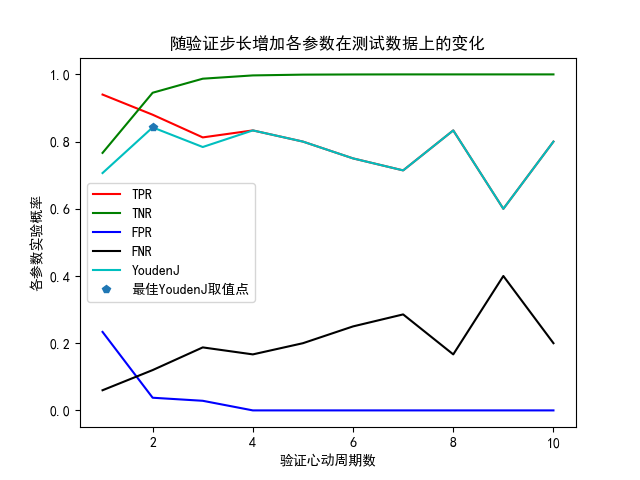
\includegraphics[width=0.7\linewidth]{images/30fps1080p.png}
  \caption{30fps1080p条件下各参数随验证所需心动周期数变化}\label{4-2} % label 用来在文中索引
\end{figure}

\par
{如图4-2所示,在心动周期数为2时取得最佳效果,此时的TPR为88\%,TNR为96.23\%。}}





\item {\bf{30fps4k}}{%30fps4k
{使用帧率为30fps和分辨率为4k的数据进行实验,在该条件下采集了70个合法用户的心波,心率为85,70个心波提取的特征经过PCA转换后得到36个特征,用于测试的受试者采集的数据信息如表4-5所示,其中志愿者1为合法用户,其他为攻击用户。}
  \begin{table*}[!ht]
    \linespread{1.5}
    \zihao{5}
	  \centering  % 显示位置为中间
	  \caption{受试者基本信息}  % 表格标题
	  \label{table4-5} 
	  %字母的个数对应列数,|代表分割线
	  % l代表左对齐,c代表居中,r代表右对齐
	  \scalebox{0.8}{\begin{tabular}{*{3}{>{\centering\arraybackslash}p{3cm}}} \toprule %l左对齐;c居中;r右对齐
	  	用户 & 心跳周期数 & 心率(单位: 次/min)   \\
	  	\hline
	  	志愿者1 & 33 & 90   \\
	  	志愿者2 & 28 & 81   \\
	  	志愿者3 & 31 & 89   \\
	  	志愿者4 & 16 & 108   \\
	  	志愿者5 & 22 & 78   \\
    \bottomrule
	  \end{tabular}}
  \end{table*}
\par
{各个评估指标在不同心动周期作为验证步长的情况下测量值如表4-6所示。}

\begin{table*}[htbp]
  \linespread{1.5}
  \zihao{5}
  \centering
  \caption{各参数实验结果统计表} 
\label{table4-6}
\scalebox{0.6}{
  \begin{tabular}{*{10}{>{\centering\arraybackslash}p{2cm}}} \toprule
  步长$n$ & 实际TPR & 理论TPR & 实际FNR & 理论FNR  & 实际TNR & 理论TNR & 实际FPR & 理论FPR & YoudenJ \\
    \hline
1&0.9394&0.9394&0.0606&0.0606&0.866&0.866&0.134&0.134&0.8054 \\ 
2&0.9375&0.8825&0.0625&0.1175&1.0&0.982&0.0&0.018&0.9375 \\ 
3&0.9091&0.829&0.0909&0.171&1.0&0.9976&0.0&0.0024&0.9091 \\ 
4&0.875&0.7787&0.125&0.2213&1.0&0.9997&0.0&0.0003 &0.875 \\ 
5&0.8333&0.7315&0.1667&0.2685&1.0&1.0&0.0&0.0&0.8333 \\ 
6&0.8&0.6872&0.2&0.3128&1.0&1.0&0.0&0.0&0.8 \\ 
7&0.75&0.6456&0.25&0.3544&1.0&1.0&0.0&0.0&0.75 \\ 
8&0.75&0.6064&0.25&0.3936&1.0&1.0&0.0&0.0&0.75 \\ 
9&0.6667&0.5697&0.3333&0.4303&1.0&1.0&0.0&0.0&0.6667 \\ 
10&0.6667&0.5352&0.3333&0.4648&1.0&1.0&0.0&0.0&0.6667 \\ 

\bottomrule
    \end{tabular}}
\end{table*}


\begin{figure}[H]
  \centering
  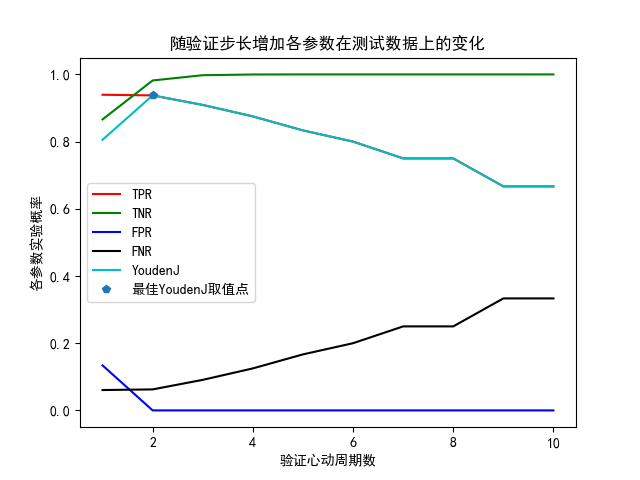
\includegraphics[width=0.7\linewidth]{images/30fps4k.png}
  \caption{30fps4k条件下各参数随验证所需心动周期数变化}\label{4-3} % label 用来在文中索引
\end{figure}
\par
{如图4-3所示,在心动周期数为2时取得最佳效果,此时的TPR为93.75\%,TNR为100\%。}
}





\item {\bf{60fps720p}}{%60fps720p
{使用帧率为60fps和分辨率为720p的数据进行实验,在该条件下采集了70个合法用户的心波,心率为83,70个心波提取的特征经过PCA转换后得到33个特征,用于测试的受试者采集的数据信息如表4-7所示,其中志愿者1为合法用户,其他为攻击用户。}
  \begin{table}[!ht]
    \linespread{1.5}
    \vspace{-0.5cm}
    \zihao{5}
	  \centering  % 显示位置为中间
	  \caption{受试者基本信息}  % 表格标题
	  \label{table4-7} 
	  %字母的个数对应列数,|代表分割线
	  % l代表左对齐,c代表居中,r代表右对齐
	  \scalebox{0.7}{\begin{tabular}{*{3}{>{\centering\arraybackslash}p{3cm}}} \toprule %l左对齐;c居中;r右对齐
	  	用户 & 心跳周期数 & 心率(单位: 次/min)   \\
	  	\hline
	  	志愿者1 & 34 & 95   \\
	  	志愿者2 & 29 & 84   \\
	  	志愿者3 & 27 & 87   \\
	  	志愿者4 & 38 & 103   \\
	  	志愿者5 & 23 & 82   \\
    \bottomrule
	  \end{tabular}}
   \vspace{-1cm}
  \end{table}
\par
{各个评估指标在不同心动周期作为验证步长的情况下测量值如表4-8所示。}

\begin{table*}[htbp]
  \linespread{1.5}
  \vspace{-0.5cm}
  \zihao{5}
  \centering
  \caption{各参数实验结果统计表} 
\label{table4-8}
\scalebox{0.6}{
  \begin{tabular}{*{10}{>{\centering\arraybackslash}p{2cm}}} \toprule
  步长$n$ & 实际TPR & 理论TPR & 实际FNR & 理论FNR  & 实际TNR & 理论TNR & 实际FPR & 理论FPR & YoudenJ \\
    \hline
1&0.8235&0.8235&0.1765&0.1765&0.7009&0.7009&0.2991&0.2991&0.5244 \\ 
2&0.6471&0.6782&0.3529&0.3218&0.9138&0.9105&0.0862&0.0895&0.5609 \\ 
3&0.5455&0.5585&0.4545&0.4415&0.9744&0.9732&0.0256&0.0268&0.5199 \\ 
4&0.375&0.46&0.625&0.54&0.9655&0.992&0.0345&0.008 &0.3405 \\ 
5&0.3333&0.3788&0.6667&0.6212&1.0&0.9976&0.0&0.0024 &0.3333 \\ 
6&0.2&0.3119&0.8&0.6881&1.0&0.9993&0.0&0.0007&0.2 \\ 
7&0.0&0.2569&1.0&0.7431&1.0&0.9998&0.0&0.0002&0.0 \\ 
8&0.25&0.2116&0.75&0.7884&1.0&0.9999&0.0&0.0001 &0.25 \\ 
9&0.0&0.1742&1.0&0.8258&1.0&1.0&0.0&0.0 &0.0 \\ 
10&0.0&0.1435&1.0&0.8565&1.0&1.0&0.0&0.0 &0.0 \\

\bottomrule
    \end{tabular}}
    \vspace{-1cm}
\end{table*}


\begin{figure}[H]
\vspace{-1cm}
  \centering
  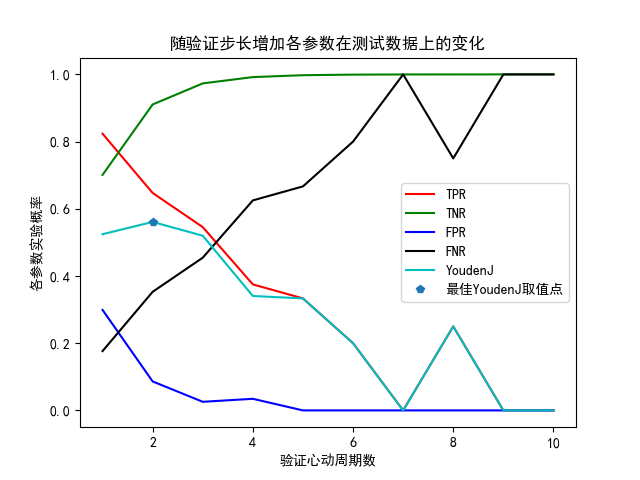
\includegraphics[width=0.7\linewidth]{images/60fps720p.png}
  \caption{60fps720p条件下各参数随验证所需心动周期数变化}\label{4-4} % label 用来在文中索引
  \vspace{-1cm}
\end{figure}
\par
{如图4-4所示,在心动周期数为2时取得最佳效果,此时的TPR为64.71\%,TNR为91.38\%。}}


\vspace{1cm}

\item {\bf{60fps1080p}}{%60fps1080p
{使用帧率为60fps和分辨率为1080p的数据进行实验,在该条件下采集了70个合法用户的心波,心率为93,70个心波提取的特征经过PCA转换后得到37个特征,用于测试的受试者采集的数据信息如表4-9所示,其中志愿者1为合法用户,其他为攻击用户。}
  \begin{table}[!ht]
    \linespread{1.5}
    \vspace{1cm}
    \zihao{5}
	  \centering  % 显示位置为中间
	  \caption{受试者基本信息}  % 表格标题
	  \label{table4-9} 
	  %字母的个数对应列数,|代表分割线
	  % l代表左对齐,c代表居中,r代表右对齐
	  \scalebox{0.8}{\begin{tabular}{*{3}{>{\centering\arraybackslash}p{3cm}}} \toprule %l左对齐;c居中;r右对齐
	  	用户 & 心跳周期数 & 心率(单位: 次/min)   \\
	  	\hline
	  	志愿者1 & 31 & 90   \\
	  	志愿者2 & 29 & 82   \\
	  	志愿者3 & 33 & 95   \\
	  	志愿者4 & 36 & 105   \\
	  	志愿者5 & 14 & 83   \\
    \bottomrule
	  \end{tabular}}
  \end{table}
\par
{各个评估指标在不同心动周期作为验证步长的情况下测量值如表4-10所示。}

\begin{table*}[htbp]
  \linespread{1.5}
  \vspace{1cm}
  \zihao{5}
  \centering
  \caption{各参数实验结果统计表} 
\label{table4-10}
\scalebox{0.6}{
  \begin{tabular}{*{10}{>{\centering\arraybackslash}p{2cm}}} \toprule
  步长$n$ & 实际TPR & 理论TPR & 实际FNR & 理论FNR  & 实际TNR & 理论TNR & 实际FPR & 理论FPR & YoudenJ \\
    \hline
1&0.7742&0.7742&0.2258&0.2258&0.9286&0.9286&0.0714&0.0714&0.7028 \\ 
2&0.6667&0.5994&0.3333&0.4006&1.0&0.9949&0.0&0.0051&0.6667 \\ 
3&0.6&0.464&0.4&0.536&1.0&0.9996&0.0&0.0004&0.6 \\ 
4&0.4286&0.3593&0.5714&0.6407&1.0&1.0&0.0&0.0&0.4286 \\ 
5&0.3333&0.2781&0.6667&0.7219&1.0&1.0&0.0&0.0&0.3333 \\ 
6&0.4&0.2153&0.6&0.7847&1.0&1.0&0.0&0.0&0.4 \\ 
7&0.25&0.1667&0.75&0.8333&1.0&1.0&0.0&0.0&0.25 \\ 
8&0.3333&0.1291&0.6667&0.8709&1.0&1.0&0.0&0.0&0.3333 \\ 
9&0.0&0.0999&1.0&0.9001&1.0&1.0&0.0&0.0&0.0 \\ 
10&0.0&0.0774&1.0&0.9226&1.0&1.0&0.0&0.0&0.0 \\ 

\bottomrule
    \end{tabular}}
\end{table*}



\begin{figure}[H]
  \centering
  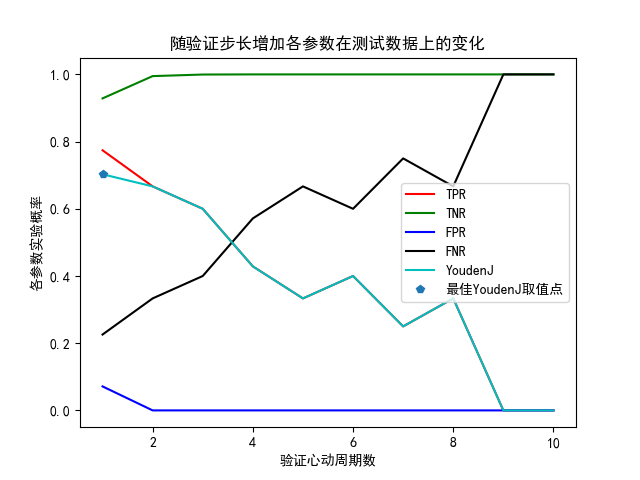
\includegraphics[width=0.7\linewidth]{images/60fps1080p.png}
  \caption{60fps1080p条件下各参数随验证所需心动周期数变化}\label{4-5} % label 用来在文中索引
\end{figure}
\par
{如图4-5所示,在心动周期数为1时取得最佳效果,此时的TPR为77.42\%,TNR为92.86\%。}}






\item {\bf{60fps4k}}{%60fps4k
{使用帧率为60fps和分辨率为4k的数据进行实验在该条件下采集了70个合法用户的心波,心率为83,70个心波提取的特征经过PCA转换后得到33个特征,用于测试的受试者采集的数据信息如表4-11所示,其中志愿者1为合法用户,其他为攻击用户。}
  \begin{table}[!ht]
    \linespread{1.5}
    \zihao{5}
	  \centering  % 显示位置为中间
	  \caption{受试者基本信息}  % 表格标题
	  \label{table4-11} 
	  %字母的个数对应列数,|代表分割线
	  % l代表左对齐,c代表居中,r代表右对齐
	  \scalebox{0.8}{\begin{tabular}{*{3}{>{\centering\arraybackslash}p{3cm}}} \toprule %l左对齐;c居中;r右对齐
	  	用户 & 心跳周期数 & 心率(单位: 次/min)   \\
	  	\hline
	  	志愿者1 & 44 & 92   \\
	  	志愿者2 & 35 & 90   \\
	  	志愿者3 & 38 & 90   \\
	  	志愿者4 & 39 & 115   \\
	  	志愿者5 & 14 & 89   \\
    \bottomrule
	  \end{tabular}}
  \end{table}
\par
{各个评估指标在不同心动周期作为验证步长的情况下测量值如表4-12所示。}

\begin{table*}[htbp]
  \linespread{1.5}
  \vspace{1cm}
  \zihao{5}
  \centering
  \caption{各参数实验结果统计表} 
\label{table4-12}
\scalebox{0.6}{
  \begin{tabular}{*{10}{>{\centering\arraybackslash}p{2cm}}} \toprule
  步长$n$ & 实际TPR & 理论TPR & 实际FNR & 理论FNR  & 实际TNR & 理论TNR & 实际FPR & 理论FPR & YoudenJ \\
    \hline
1&0.8636&0.8636&0.1364&0.1364&0.7857&0.7857&0.2143&0.2143&0.6493 \\ 
2&0.7727&0.7459&0.2273&0.2541&0.9365&0.9541&0.0635&0.0459&0.7092 \\ 
3&0.6429&0.6442&0.3571&0.3558&0.9762&0.9902&0.0238&0.0098&0.6191 \\ 
4&0.5455&0.5563&0.4545&0.4437&1.0&0.9979&0.0&0.0021&0.5455 \\ 
5&0.25&0.4805&0.75&0.5195&1.0&0.9995&0.0&0.0005&0.25 \\ 
6&0.4286&0.4149&0.5714&0.5851&1.0&0.9999&0.0&0.0001 &0.4286 \\ 
7&0.3333&0.3584&0.6667&0.6416&1.0&1.0&0.0&0.0&0.3333 \\ 
8&0.2&0.3095&0.8&0.6905&1.0&1.0&0.0&0.0&0.2 \\ 
9&0.0&0.2673&1.0&0.7327&1.0&1.0&0.0&0.0&0.0 \\ 
10&0.0&0.2308&1.0&0.7692&1.0&1.0&0.0&0.0&0.0 \\ 
 
\bottomrule
    \end{tabular}}
\end{table*}


\begin{figure}[H]
\vspace{1cm}
  \centering
  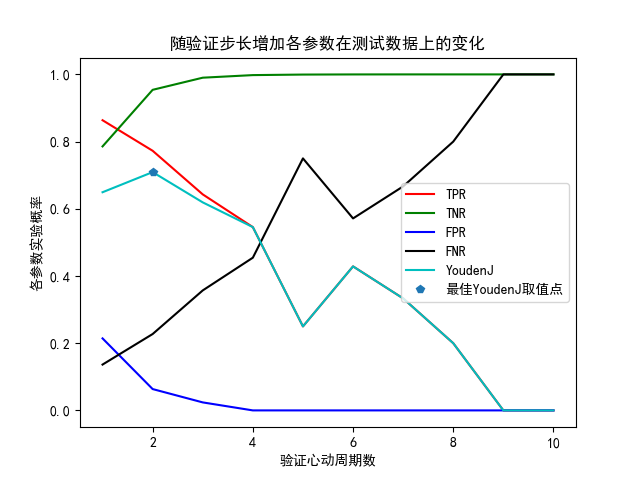
\includegraphics[width=0.7\linewidth]{images/60fps4k.png}
  \caption{60fps4k条件下各参数随验证所需心动周期数变化}\label{4-6} % label 用来在文中索引
\end{figure}
\par
{如图4-6所示,在心动周期数为2时取得最佳效果,此时的TPR为77.27\%,TNR为93.65\%。}}

\end{itemize}
\par
{从上述不同帧率与分辨率的实验效果看,大多数情况下验证2个心动周期即能达到较好下效果,我们对比在2个心动周期进行验证的情况下不同分辨率与帧率的效果,如表4-13所示。}
\begin{table}[H]
  \linespread{1.5}
  \zihao{5}
  \centering
  \caption{各参数实验结果统计表} 
\label{table4-13}
% \scalebox{0.8}{
  \begin{tabular}{c|cc|cc|cc} \toprule
  &\multicolumn{2}{c|}{ 720p} &\multicolumn{2}{c|}{ 1080p} &\multicolumn{2}{c}{ 4k}   \\
  \hline
  帧率 & TPR & TNR & TPR & TNR & TPR & TNR \\
  \hline
  30 & 68.75\% & 95.83\% & 88\% & 96.23\% & 93.75\% & 100\% \\
  60 & 64.71\% & 91.83\% & 66.67\% & 100\% & 77.27\% & 93.65\% \\
\bottomrule
    \end{tabular}
    % }
\end{table}
{由表4-13可知,帧率的提升对系统性能几乎没有任何影响,而分辨率的提高明显提升了在测试数据集上的TPR和TNR测量值,能明显提升性能。考虑道4k的分辨率不是所有设备都能满足,而30fps与1080p的分辨率已经具有较好的系统性能,因此选择帧率为30fps与分辨率为1080p的配置作为标准进行后续测试。}











\subsection{不同手指的准确率分析}
{我们将食指按压生成的配置文件用于测试中指按压的测试数据,又使用中指按压生成的配置文件用于测试食指按压的测试数据。先选取上一节的帧率为30fps,分辨率为1080p的食指按压数据生成配置文件用于匹配。使用中指按压,选择帧率为30fps和分辨率为1080p的摄像头配置采集测试者数据,用于测试的受试者采集的数据信息如表4-14所示,其中志愿者1为合法用户,其他为攻击用户。}


  \begin{table}[H]
    \linespread{1.5}
    \zihao{5}
	  \centering  % 显示位置为中间
	  \caption{受试者基本信息}  % 表格标题
	  \label{table4-14} 
	  %字母的个数对应列数,|代表分割线
	  % l代表左对齐,c代表居中,r代表右对齐
	  \begin{tabular}{*{3}{>{\centering\arraybackslash}p{3cm}}} \toprule %l左对齐;c居中;r右对齐
	  	用户 & 心跳周期数 & 心率(单位: 次/min)   \\
	  	\hline
	  	志愿者1 & 38 & 92   \\
	  	志愿者2 & 22 & 84   \\
	  	志愿者3 & 56 & 91   \\
	  	志愿者4 & 33 & 97   \\
	  	志愿者5 & 19 & 77   \\
    \bottomrule
	  \end{tabular}
   \vspace{0.5cm}
  \end{table}

\par
{各个评估指标在不同心动周期作为验证步长的情况下测量值如表4-15所示。}
\begin{table*}[htbp]
  \linespread{1.5}
  \vspace{1cm}
  \zihao{5}
  \centering
  \caption{各参数实验结果统计表} 
\label{table8-2}
\scalebox{0.6}{
  \begin{tabular}{*{10}{>{\centering\arraybackslash}p{2cm}}} \toprule
  步长$n$ & 实际TPR & 理论TPR & 实际FNR & 理论FNR  & 实际TNR & 理论TNR & 实际FPR & 理论FPR & YoudenJ \\
    \hline
1&0.1842&0.5&0.8158&0.5&0.6692&0.9231&0.3308&0.0769&-0.1466 \\ 
2&0.0526&0.25&0.9474&0.75&0.8615&0.9941&0.1385&0.0059&-0.0859 \\ 
3&0.0&0.125&1.0&0.875&0.9767&0.9995&0.0233&0.0005&-0.0233 \\ 
4&0.0&0.0625&1.0&0.9375&1.0&1.0&0.0&0.0&0.0 \\ 
5&0.0&0.0312&1.0&0.9688&1.0&1.0&0.0&0.0&0.0 \\ 
6&0.0&0.0156&1.0&0.9844&1.0&1.0&0.0&0.0&0.0 \\ 
7&0.0&0.0078&1.0&0.9922&1.0&1.0&0.0&0.0&0.0 \\ 
8&0.0&0.0039&1.0&0.9961&1.0&1.0&0.0&0.0&0.0 \\ 
9&0.0&0.002&1.0&0.998&1.0&1.0&0.0&0.0&0.0 \\ 
10&0.0&0.001&1.0&0.999&1.0&1.0&0.0&0.0&0.0 \\ 
\bottomrule
    \end{tabular}}
\end{table*}


\begin{figure}[H]
  \centering
  \vspace{0.5cm}
  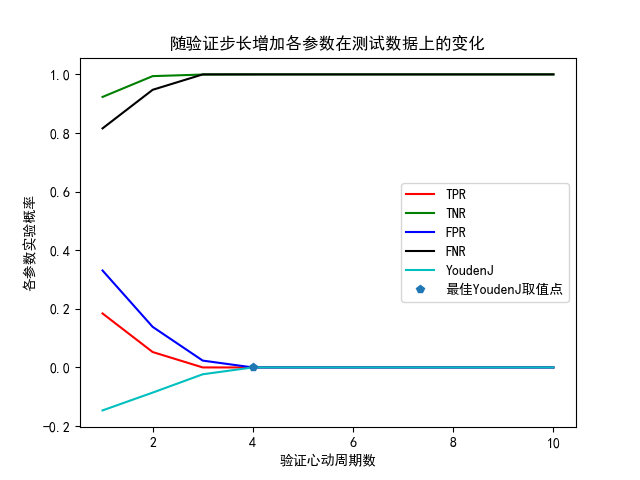
\includegraphics[width=0.7\linewidth]{images/shizhi.png}
  \caption{中指按压条件下各参数随验证所需心动周期数变化}\label{4-7} % label 用来在文中索引
\end{figure}
\par
{如图4-7所示,在心动周期数为4时取得最大YoudenJ值,但是此时的TPR为0.0\%,TNR为100\%。}
\par
{使用中指按压,选择帧率为30fps和分辨率为1080p的配置进行实验,在该条件下采集了70个合法用户的心波,心率为91,70个心波提取的特征经过PCA转换后得到35个特征,选择食指按压的帧率为30fps和分辨率为1080p数据进行测试,采集的测试数据信息在上一节已经给出。}

\par

{各个评估指标在不同心动周期作为验证步长的情况下测量值如表4-16所示。}
\begin{table*}[htbp]
  \linespread{1.5}
  \zihao{5}
  \centering
  \caption{各参数实验结果统计表} 
\label{table4-16}
\scalebox{0.6}{
  \begin{tabular}{*{10}{>{\centering\arraybackslash}p{2cm}}} \toprule
  步长$n$ & 实际TPR & 理论TPR & 实际FNR & 理论FNR  & 实际TNR & 理论TNR & 实际FPR & 理论FPR & YoudenJ \\
    \hline
1&0.86&0.86&0.14&0.14&0.7664&0.7664&0.2336&0.2336&0.6264 \\ 
2&0.72&0.7396&0.28&0.2604&0.9623&0.9454&0.0377&0.0546&0.6823 \\ 
3&0.625&0.6361&0.375&0.3639&1.0&0.9872&0.0&0.0128&0.625 \\ 
4&0.5833&0.547&0.4167&0.453&1.0&0.997&0.0&0.003&0.5833 \\ 
5&0.5&0.4704&0.5&0.5296&1.0&0.9993&0.0&0.0007&0.5 \\ 
6&0.5&0.4046&0.5&0.5954&1.0&0.9998&0.0&0.0002&0.5 \\ 
7&0.5714&0.3479&0.4286&0.6521&1.0&1.0&0.0&0.0&0.5714 \\ 
8&0.3333&0.2992&0.6667&0.7008&1.0&1.0&0.0&0.0&0.3333 \\ 
9&0.4&0.2573&0.6&0.7427&1.0&1.0&0.0&0.0&0.4 \\ 
10&0.4&0.2213&0.6&0.7787&1.0&1.0&0.0&0.0&0.4 \\ 

\bottomrule
    \end{tabular}}
\end{table*}


\begin{figure}[H]
  \centering
  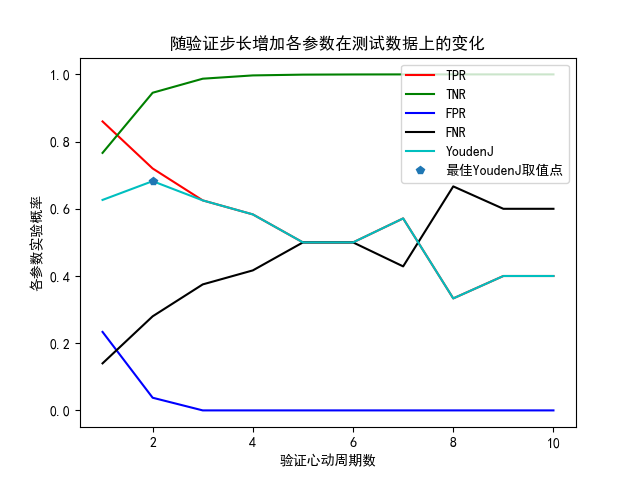
\includegraphics[width=0.7\linewidth]{images/zhongzhi.png}
  \caption{食指按压条件下各参数随验证所需心动周期数变化}\label{4-8} % label 用来在文中索引
\end{figure}
\par
{如图4-8所示,在心动周期数为2时取得最佳效果,此时的TPR为72\%,TNR为96.23\%。}
\par
{进行交叉测试后我们发现,在取2个心动周期进行验证时,中指按压的数据作为测试数据的测试结果不太理想,当取3个心动周期进行验证时才具有较高的TNR,但是TPR一直很低,对于验证效率影响巨大。而对于食指按压的数据作为测试数据的一组具有较好的表现,但是TPR依旧较低。由此说明不同手指进行用户身份认证对于系统拒绝非法用户的功能无太大影响,但对于合法用户进行验证的效率会大打折扣,即系统对合法用户和非法用户的特征识别度降低。}












